%&pdflatex
\documentclass{standalone}
    \usepackage{tikz}
    \usetikzlibrary{backgrounds}
    \usepackage{graphicx}

    \pagenumbering{gobble}
    
% Some customizable styles
    \tikzset {
        highlight/.style = {gray, opacity=0.3},
        digit/.style = {minimum height = 5mm, minimum width=5mm, anchor=center },
        circle/.style = {draw=black!80!black, dotted, very thick},
        cross/.style = {red, opacity=.5, shorten >=1mm, shorten <=1mm, very thick, line cap=round},
        hint/.style={black, font=\sf, minimum width=3mm, minimum height=3mm}
    }

% Original code-----------------------------------------------------------
% Modified the \node to give a unique name to each one, which is the
% row number, a dash and the column number. E.g: 1-1, 4-5, etc.
    \newcounter{row}
    \newcounter{col}

    \newcommand\setrow[9]{
        \setcounter{col}{1}
        \foreach \n in {#1, #2, #3, #4, #5, #6, #7, #8, #9} {
            \edef\x{\value{col} - 0.5}
            \edef\y{9.5 - \value{row}}
            \node[digit,name={\arabic{row}-\arabic{col}}] at (\x, \y) {\n};
            \stepcounter{col}
        }
        \stepcounter{row}
    }

% New code -------------------------------------------------------------
    \def\highlightcell#1#2{
        \fill[highlight] (#1-#2.north west) rectangle (#1-#2.south east);
    }

    \def\circlecell#1#2{
        \draw[circle] (#1-#2) circle(4mm);
    }

    \def\crosscell#1#2{
        \draw[cross] (#1-#2.north west) -- (#1-#2.south east);
        \draw[cross] (#1-#2.north east) -- (#1-#2.south west);
    }

    \def\highlightrow#1{
       \fill[highlight] (#1-1.north west) rectangle (#1-9.south east);
    }

    \def\highlighcolumn#1{
        \fill[highlight] (1-#1.north west) rectangle (9-#1.south east);
    }

    \def\hintcell#1#2#3{
        \node at (#1-#2) {\hintbox{#3}};
    }

    \def\highlightrectangle#1#2#3#4{
        \begin{pgfonlayer}{background}
        \fill[highlight] (#1-#2.north west) rectangle (#3-#4.south east);
        \end{pgfonlayer}
    }

% UGLY code. Do not read :-)
\def\hintbox#1{
    \resizebox{4.5mm}{4.5mm}{%
        \tikz[scale=0.3]{%
            \def\auxc{0}
            \foreach \m in {1,...,9} {
                \pgfmathparse{mod(\auxc,3)}
                \xdef\x{\pgfmathresult}
                \pgfmathparse{-floor(\auxc/3)}
                \xdef\y{\pgfmathresult}
                \xdef\hintprinted{0}
                \foreach \n in {#1} {
                    \ifnum\n=\m
                        \node[hint] at (\x,\y) {\n};
                        \xdef\hintprinted{1}
                    \fi
                }
                \ifnum\hintprinted=0
                      \node[hint, opacity=0] at (\x,\y) {\m};
                \fi
                \pgfmathparse{\auxc+1}
                \xdef\auxc{\pgfmathresult}
            }
        }%
    }
}


\begin{document}
    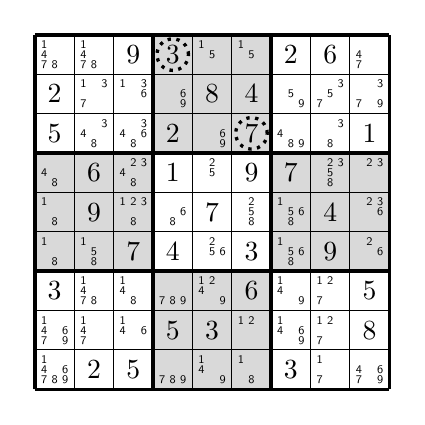
\begin{tikzpicture}[scale=.5]
        \begin{scope}
            \draw (0, 0) grid (9, 9);
            \draw[very thick, scale=3] (0, 0) grid (3, 3);
            \setcounter{row}{1}

    % Single entries
            \setrow { }{ }{9}  {3}{ }{ }  {2}{6}{ }
            \setrow {2}{ }{ }  { }{8}{4}  { }{ }{ }
            \setrow {5}{ }{ }  {2}{ }{7}  { }{ }{1}

            \setrow { }{6}{ }  {1}{ }{9}  {7}{ }{ }
            \setrow { }{9}{ }  { }{7}{ }  { }{4}{ }
            \setrow { }{ }{7}  {4}{ }{3}  { }{9}{ }

            \setrow {3}{ }{ }  { }{ }{6}  { }{ }{5}
            \setrow { }{ }{ }  {5}{3}{ }  { }{ }{8}
            \setrow { }{2}{5}  { }{ }{ }  {3}{ }{ }

            \circlecell{1}{4}
            \circlecell{3}{6}

            \highlightrectangle{1}{4}{3}{6}

            \highlightrectangle{4}{1}{6}{3}
            \highlightrectangle{4}{7}{6}{9}
            
            \highlightrectangle{7}{4}{9}{6}
            % Hints
    %  * Row 1
            \hintcell{1}{1}{1,4,7,8}
            \hintcell{1}{2}{1,4,7,8}
            \hintcell{1}{5}{1,5}
            \hintcell{1}{6}{1,5}
            \hintcell{1}{9}{4,7}
    %  * Row 2
            \hintcell{2}{2}{1,3,7}
            \hintcell{2}{3}{1,3,6}
            \hintcell{2}{4}{6,9}
            \hintcell{2}{7}{5,9}
            \hintcell{2}{8}{3,5,7}
            \hintcell{2}{9}{3,7,9}
    %  * Row 3
            \hintcell{3}{2}{3,4,8}
            \hintcell{3}{3}{3,4,6,8}
            \hintcell{3}{5}{6,9}
            \hintcell{3}{7}{4,8,9}
            \hintcell{3}{8}{3,8}
    %  * Row 4
            \hintcell{4}{1}{4,8}
            \hintcell{4}{3}{2,3,4,8}
            \hintcell{4}{5}{2,5}
            \hintcell{4}{8}{2,3,5,8}
            \hintcell{4}{9}{2,3}
    %  * Row 5
            \hintcell{5}{1}{1,8}
            \hintcell{5}{3}{1,2,3,8}
            \hintcell{5}{4}{6,8}
            \hintcell{5}{6}{2,5,8}
            \hintcell{5}{7}{1,5,6,8}
            \hintcell{5}{9}{2,3,6}
    %  * Row 6
            \hintcell{6}{1}{1,8}
            \hintcell{6}{2}{1,5,8}
            \hintcell{6}{5}{2,5,6}
            \hintcell{6}{7}{1,5,6,8}
            \hintcell{6}{9}{2,6}
    %  * Row 7
            \hintcell{7}{2}{1,4,7,8}
            \hintcell{7}{3}{1,4,8}
            \hintcell{7}{4}{7,8,9}
            \hintcell{7}{5}{1,2,4,9}
            \hintcell{7}{7}{1,4,9}
            \hintcell{7}{8}{1,2,7}
    %  * Row 8
            \hintcell{8}{1}{1,4,6,7,9}
            \hintcell{8}{2}{1,4,7}
            \hintcell{8}{3}{1,4,6}
            \hintcell{8}{6}{1,2}
            \hintcell{8}{7}{1,4,6,9}
            \hintcell{8}{8}{1,2,7}
    %  * Row 9
            \hintcell{9}{1}{1,4,6,7,8,9}
            \hintcell{9}{4}{7,8,9}
            \hintcell{9}{5}{1,4,9}
            \hintcell{9}{6}{1,8}
            \hintcell{9}{8}{1,7}
            \hintcell{9}{9}{4,6,7,9}
        \end{scope}
\end{tikzpicture}

\end{document}
